% ---------------------------------------------------------------------
% EG author guidelines plus sample file for EG publication using LaTeX2e input
% D.Fellner, v2.02, Jan 25, 2017


\title[ParamNet: Towards A Network of \emph{Parameterization
	Prediction} for Shape Generation from a Single Image]%
      {ParamNet: Towards A Network of \emph{Parameterization
      	Prediction} for Shape Generation from a Single Image}

% for anonymous conference submission please enter your SUBMISSION ID
% instead of the author's name (and leave the affiliation blank) !!
\author[ID: paper1147]
{ID: paper1147}
% ------------------------------------------------------------------------

% if the Editors-in-Chief have given you the data, you may uncomment
% the following five lines and insert it here
%
% \volume{36}   % the volume in which the issue will be published;
% \issue{1}     % the issue number of the publication
% \pStartPage{1}      % set starting page


%-------------------------------------------------------------------------
\begin{document}

% uncomment for using teaser
% \teaser{
%  \includegraphics[width=\linewidth]{eg_new}
%  \centering
%   \caption{New EG Logo}
% \label{fig:teaser}
%}

\maketitle
%-------------------------------------------------------------------------
\begin{abstract}
	We propose an end-to-end deep learning framework that maps from a unit sphere surface to the target surface, given a single color image. 
	%Previous methods usually represent a 3D shape in volume or point cloud, and it is non-trivial to convert them to mesh models which are ready for wider application. 
	While mesh or surface models are widely used in many applications, it is challenging to apply the successful deep neural networks to directly produce surface models.  
	Unlike the methods that use volumetric or point representations, our method represents a 3D shape by a mapping from a fixed parameter domain. 
	%
	In our framework, the mapping is progressively carried out by the \emph{parameterization network}, given parameters that are predicted by the \emph{semantic network} from a single color image. 
	%
	By integrating mesh-based operation (e.g. Laplacian smooth) and mesh related losses into the network, our framework directly outputs high-quality meshes.
	Experiments show that our method not only produces mesh models that are more visually appealing, but also achieves comparable 3D shape estimation errors compared to the state of the art.
	%-------------------------------------------------------------------------
	%  ACM CCS 1998
	%  (see http://www.acm.org/about/class/1998)
	% \begin{classification} % according to http:http://www.acm.org/about/class/1998
	% \CCScat{Computer Graphics}{I.3.3}{Picture/Image Generation}{Line and curve generation}
	% \end{classification}
	%-------------------------------------------------------------------------
	%  ACM CCS 2012
	%(see http://www.acm.org/about/class/class/2012)
	%The tool at \url{http://dl.acm.org/ccs.cfm} can be used to generate
	% CCS codes.
	%Example:
	\begin{CCSXML}
	<ccs2012>
	<concept>
	<concept_id>10010147.10010178.10010224.10010240.10010242</concept_id>
	<concept_desc>Computing methodologies~Shape representations</concept_desc>
	<concept_significance>500</concept_significance>
	</concept>
	<concept>
	<concept_id>10010147.10010257.10010293.10010294</concept_id>
	<concept_desc>Computing methodologies~Neural networks</concept_desc>
	<concept_significance>500</concept_significance>
	</concept>
	<concept>
	<concept_id>10010147.10010371.10010396.10010397</concept_id>
	<concept_desc>Computing methodologies~Mesh models</concept_desc>
	<concept_significance>500</concept_significance>
	</concept>
	</ccs2012>
	\end{CCSXML}

	\ccsdesc[500]{Computing methodologies~Shape representations}
	\ccsdesc[500]{Computing methodologies~Neural networks}
	\ccsdesc[500]{Computing methodologies~Mesh models}
	
	
	\printccsdesc  
\end{abstract} 
%-------------------------------------------------------------------------
\section{Introduction}
\begin{figure}[htbp]
	\centering
	\includegraphics[width=\linewidth]{img/issue/issue}
	\caption{(a) The issue of the self-intersected surface in 3D surface mesh reconstruction networks: (a) A surface mesh of plane generated by Pixel2Mesh \cite{pixel2mesh}. (b) A surface mesh of plane generated by AtlasNet \cite{atlasnet}(sphere as parameter domain). The triangle faces are rendered as golden on outside and bluish on inside. The inside color is exposed due to the issue of self-intersection. Some examples of the issue are also highlighted in zoomed view}
	\label{fig:issue}
\end{figure}
%introduction to 3D shape reconstruction from single view
Inferring 3D shape from a single view image is a traditional problem for computer vision. In computer graphics, 3D modeling with a given image has also been extensively studied. In recent years, deep neural networks (e.g. \cite{3DR2N2,PSGN,3Drender,imgrecon15,3dshapenet,endface,octreegen,surfnet,shapeprior}) have achieved great success in this field. Unlike classic shape from X (e.g. \cite{shapefromshading,shapefromtext1,shapefromtext2}) approaches, these neural networks are able to recover not only the visible frontal shape but also the invisible part for object from a single view color image by learning complicate prior knowledge from dataset. 

These networks all rely on variants of 2D convolution neural network to extract information and encode 2D images, but use quite different techniques to represent and decode 3D shapes. Started by 3D ShapeNets \cite{3dshapenet} and greatly improved by introducing octree structure \cite{octreegen}, volumetric representation and 3D convolution networks are most commonly used in this problem. There is also point set generation network \cite{PSGN} that use unordered point set representation and directly regress point set using both convolution and fully connected branches. Other approaches include \cite{endface} which use bilinear model to represent shape of face and regress the interpolation coefficient to generate the shape and \cite{surfnet} which explicitly employ spherical parameterization as post-processing to represent shape as geometry image in parameter domain and so on.

%introduction to 3d mesh reconstruction networks-- AtlasNet and Pixel2Mesh to be specific
In latest works, AtlasNet \cite{atlasnet} and Pixel2Mesh \cite{pixel2mesh} to be specific, a new idea have been applied on this problem, which let the network learns to map from a predefined surface (square and sphere for AtlasNet and ellipsoid for Pixel2Mesh) to target surface instead of directly regress the absolute positions of surface points as in \cite{PSGN}. These methods have shown great potential in generating meshes for generic objects. It is convenient to integrate mesh-related operations and energy functions in these networks (The graph-based unpooling and Laplacian regularization term from Pixel2Mesh are examples of such integration).

%introduction to the self-intersection issue
In this paper, we address a specific issue that appears in both AtlasNet \cite{atlasnet} and Pixel2Mesh \cite{pixel2mesh}. As shown in Figure~\ref{fig:issue}, the AtlasNet and Pixel2Mesh will generate mesh with self-intersected surface. This issue appears partially because AtlasNet and Pixel2Mesh employed the Chamfer distance loss from point set generation network (PSGN \cite{PSGN}). The Chamfer distance loss was designed to measure the discrepancy between two unordered point set and it does not take surface into consideration. The AtlasNet used Poission surface reconstruction as post-processing or double-sided lighting in rendering to cover this issue. The Pixel2Mesh have adopted coarse-to-fine framework and added several other losses (i.e. edge length loss, Laplacian loss) that help to alleviate this issue. They all failed to address the essential reason behind this issue, after all most effort in previous mesh generation networks have been focused on increasing shape details for the generated mesh.

In this paper, we tackle the issue of self-intersection from the essential reason behind it, which is the non-injectivity of the predicted mapping, or in other words, two points on the predefined surface can be mapped to same point by the neural network, causing the generated surface to be self-intersected and self-overlapped. (as we will establish in Sec~\ref{subsec:inj})

%challenge
Constraining the Jacobian of the mapping is used to enforce injectivity. \cite{tvcgprevent} have sucessfully used it to prevent self-intersection in Free-Form Deformation(FFD). Starting from an object that is free from self-intersection, \cite{tvcgprevent} devide FFD into injective sub-steps to ensure the output to be free from self-intersection.

Injectivity has also been studied under parameterization optimization to prevent folding. For surface with disk topology, one possible strategy is also to start from a feasible solution (by Tutte's embedding \cite{tutte} or its variants) and keep every optimization iteration or deformation inside feasible region. This can be enforced by adding barrier energy from distortion metrics (e.g. \cite{provableplanarmapping,lifted_bijection}), bounding the triangle distortion (e.g.\cite{freeboundary,boundeddistortion})
or using a progressive strategy \cite{Liu_PP_2018}. 

We find it difficult to adopt the strategy in these classic works into training neural networks, since the network is simultaneously learning to predict the mapping for many different shapes and only a batch of these shapes are sampled from the dataset in each training iteration. It is not easy to initialize the network parameters to ensure that initial outputs are free of self-intersection for all possible inputs. It is also not easy to alter batch-based optimizer to constrain the deformation of outputs to be inside injective region for all possible inputs. We propose to use regularization technique to help enforcing the learning of injective mapping for mesh. Our technique is easy to implement for neural network by reusing the existing differentiable layers, given an existing surface mesh reconstruction networks as AtlasNet \cite{atlasnet} and Pixel2Mesh \cite{pixel2mesh}.

%our solution
 Our strategy is to use an additional inverse 3D decoder to learn to predict an inverse mapping from target surface back to the predefined surface along with the forward mapping in the original network. Therefore, a point from predefined surface can be mapped to target surface and then mapped back. We use difference after such cycle mapping to form our regularization term and we call it cycle regularization. While the network learning a mapping to approach the target surface, our regularization term is trying to ensure that an inverse mapping exists (i.e making the forward mapping injective, as we explain in Sec~\ref{subsec:cyclereg}).
Note that the inverse 3D decoder is only needed in training phase, therefore it is only a part of the regularization technique and do not increase the complexity of the original neural network.

In summary, our contributions in this paper are:
\begin{itemize}
	\item We propose the cycle regularization technique to handle the surface self-intersection for surface mesh reconstruction networks. 
	\item We apply our cycle regularization technique on two latest mesh generation networks AtlasNet \cite{atlasnet} and Pixel2Mesh \cite{pixel2mesh}, showing that our technique keeps the network end-to-end trainable by using existing differentiable layers.
	\item We validate with experiments that when trained with cycle regularization these networks are able to produce surface meshes with significantly less self-intersection and keep being close to target surface by the measure of Chamfer distance.
\end{itemize}

 
%-------------------------------------------------------------------------
\begin{figure}[t]
	\centering
	\includegraphics[width=\linewidth]{img/net/net}
	\caption{The cycle regularization implemented along with networks. (a) is the implementation with AtlasNet \cite{atlasnet}. $f$ is the forward 3D surface decoder in original network and $g$ is our inverse decoder used to form the regularization term. (b) is the implementation with Pixel2Mesh \cite{pixel2mesh}.  Pixel2Mesh \cite{pixel2mesh} adopt the coarse-to-fine framework and use three \emph{G-ResNet} block ($f_1,f_2,f_3$) to map the mesh to target shape on three different point density. The \emph{Graph -Unpooling} layers are used to do the upsampling. We use three point-wise MLP ($g_1,g_2,g_3$) as inverse decoders for each level of point density and form a regularization term for each level.}
	\label{fig:net}
\end{figure}

\section{Related Work}
3D reconstruction and modeling from a single image has been extensively studied as the problem of \emph{shape from monocular cues}, including shadings~\cite{shapefromshadingsurvey}, focuses~\cite{shapefromdf1,shapefromdf2}, and textures~\cite{Aloimonos1988}. 
These methods usually recover 2.5D surfaces from 2D images. 
Learning-based approaches, especially deep learning methods, can acquire more complicated priors by learning from datasets and recover much more complete 3D shape from a single image.
 
\subsection{General Learning Approaches}
As far as we known, early work of learning approaches can be traced back to \cite{Hoiem2007} and \cite{learn3D2007}. These methods learn to segment and classify regions in an image and finally produce a coarse 3D scene by folding the 2D image.
%
More recent techniques break down the problem to two stages \cite{Su:2014,jointimgshape}. They first retrieve shape components from a large dataset, and then assemble the components and deform the assembled shape to fit the observed image. These methods need to segment the shape into components for the database.
%
However, shape retrieval from images itself is an challenging problem due to the loss of information during 3D-to-2D projection. 
\cite{imgrecon15} avoid the retrieval step by learning a deformable 3D shape for each category and learn to predict deformation from input image for these specific categories.
%
%These learning approaches are relatively early.
%A more ideal solution would be to directly learn 3D shapes from single images under an end-to-end framework.
\subsection{3D Neural Networks}
Most recently, researchers have developed techniques to represent 3D shapes inside deep learning frameworks. Unlike images, 3D shapes are not canonical functions on well-organized grids.
This leads to exploration on various representations of 3D shapes.

\noindent\textbf{Volume Occupancy}. 
An intuitive way to apply convolutional network in 3D is to use volume occupancy of regular 3D grids to represent 3D shapes~\cite{3dshapenet}. It is subsequently used for 3D shape generation~\cite{3DR2N2,learnobj}.
%
The main disadvantage of volumetric representation was the large memory consumption due to the raising of dimension when extending 2D grids to 3D. 
Octree representation is proposed to support higher resolution outputs with limited memory, and used for shape generation~\cite{octreegen} and shape analysis~\cite{ocnn}.
%The most recent work of use an octree representation for shape generation (similar representation is used in for 3D shape classification and segmentation by \cite{ocnn}), which allows to higher resolution outputswith limited memory.

\noindent\textbf{Point Cloud}. 
Compared to regular 3D grids, point clouds is not limited by fixed local connections.
Many networks have been proposed to take unordered 3D point sets as input and extract geometric features from 3D point set for classification or segmentation~\cite{pointnet,NIPS2017_7095,pointcnn}.
%
The first attempt to generate a set of discrete points from a single image using neural networks was made by \cite{PSGN}. However, it is non-trivial to construct continuous surface models from the predicted point sets, since the local variation of point positions are not continuous in the predicted point sets.

\noindent\textbf{Mesh}.
Meshes are widely used in game and movie industries.
In addition to vertex positions, the mesh representation contains local structure of vertices. 
However, mesh representation is not well supported in current neural networks.
% 
To generate mesh models using neural networks, composition weights of a series of base meshes are predicted by networks \cite{img2mesh} and \cite{endface}. %produce meshes by linear interpolating base meshes. 
Since it is only possible to choose or learn base meshes for a specific class of object, these two networks only generate meshes for a specific class of objects, such as face.
%
In comparison, the idea of learning to map from predefined domain as in AtlasNet  \cite{atlasnet} and Pixel2Mesh \cite{pixel2mesh}, can generate surface meshes for generic objects. Our work is a follow-up of their general idea and addresses a specific issue of surface self-intersection in their networks.
%but it .

\subsection{Parameterization for Neural Networks}
The idea of utilizing surface parameterization for neural networks has been explored by \cite{surfnet,geoimg}. 
Typically, a non-trainable procedure is involved for the creation of geometry image. 
Manifold surfaces are required as training data so that the shapes can be parameterized using spherical parameterization and turned into geometry image. However, the public datasets like ShapeNet \cite{shapenetdata} contain meshes that are not manifold surfaces. 
In comparison, we are seeking techniques that can be integrated into networks and can be trained end-to-end along with the networks. For the issue we are addressing, our idea is based on the same insight (self-intersection for surface mesh is related to non-injective mapping) as the parameterization techniques (e.g.\cite{provableplanarmapping,lifted_bijection,freeboundary,boundeddistortion,Liu_PP_2018}). But we propose a novel technique that is more suitable for training neural networks in an end-to-end manner. 

\subsection{Cycle Neural Networks}
The general idea of using neural networks to map from one domain to a target domain and then map back have been utilized in previous works. CycleGAN \cite{CycleGAN2017} is a famous example of such work. In CycleGAN \cite{CycleGAN2017}, the cycle relation provides an extra constraint for translating between unpaired data from different domains. In comparison, our work uses the same general idea to enforce injectivity for 3D surface mesh generation networks and trying to prevent self-intersection in generated meshes. 

\subsection{Self Intersection Removal}
The classic methods (e.g. \cite{edgeswap,removeoffset}) follow the pipeline that they first identify the self-intersected faces and then altering the faces with their proposed method. However, it is difficult to integrate such a pipeline into networks or to formulate their alterations in a differentiable manner.\\


%-------------------------------------------------------------------------
\section{Techniques and building blocks}
In this section, we will elaborate on the techniques and building blocks that we have explored for the surface decoder. 
\subsection{Association techniques}
Association techniques are used to associate the image representation $\vec{x}$ with each point $\vec{z}_{n={0,1,\dots,N}}$ from $\mathbf{Z}=[\vec{z_0},\vec{z_1},\dots,\vec{z_N}]$ that are 2D or 3D coordinates corresponding to the samples from parameter domain.

\noindent\textbf{duplicate + concatenate}
this is most intuitive choice of association techniques and have been used in AtlasNet\cite{atlasnet} and FoldingNet\cite{foldingnet}

\begin{equation}
ass(\vec{x},\mathbf{Z})=\left[
\begin{aligned}
~&\vec{z_0},&\vec{z_1},\dots,&\vec{z_N}\\
~&\vec{x}  ,&\vec{x}~,\dots,&\vec{x}
\end{aligned}
\right].
\end{equation}

\noindent\textbf{duplicate + outer-product} 
Inspired by the success of bilinear pooling, we use duplicate + outer-product as a new association technique for surface decoder. 

\begin{equation}
ass(\vec{x},\mathbf{Z})=\left[
~\\vec(\vec{z}_0\vec{x}^T),\\vec(\vec{z}_1\vec{x}^T),\dots,\\vec(\vec{z}_N\vec{x}^T)\\
\right],
\end{equation}in which, $\\vec(\mathbf{X})$ means vectorization of matrix $\mathbf{X}$ by concatenating its columns.

\noindent\textbf{\emph{K}-neighbor point convolution}
\begin{equation}
ass(\vec{x},\mathbf{Z})=\vec{b}(\vec{x})+[ \mathbf{W}(\vec{x})\mathbf{K}(\vec{z}_0),\dots,\mathbf{W}(\vec{x})\mathbf{K}(\vec{z}_N)],
\end{equation}
in which, $\mathbf{W}(\vec{x})$ is a $od \times k$ matrix depending on input image feature $\vec{x}$, it is the convolution kernel for point convolution derived from the $\vec{x}$. In implementation, $\mathbf{W}(\vec{x})$ is implemented as two fully connected layers plus a reshape operation to reshape output to $od \times k$. $\vec{b}(\vec{x})$ is a $od$ vector depending on input image feature $\vec{x}$. It is the bias for point convolution and be implemented in a similar way with $\mathbf{W}(\vec{x})$.

\subsection{Blocks for point-wise decoding}

\noindent\textbf{MLP} as a building block for point-wise decoding, its difference with usual MLP in the image classification networks is that it processing input features in a point-wise manner instead of a image-wise manner. In other words, each associated feature corresponding to a sample point from parameter domain is mapped to one 3D point by the MLP. In practice, it is easier to implement such MLP as 1x1 convolution layers than as fully connected layers.

\noindent\textbf{\emph{K}-neighbor point convolution}

\subsection{Laplace smooth layer}

\section{Network structures}

%-------------------------------------------------------------------------
\section{Experiments}

\noindent{\textbf{Data}} To show the effect of cycle regularization we use the data released by AtlasNet and Pixel2Mesh respectively \cite{3DR2N2}
\todo{explain the data we use in experiment}

\noindent{\textbf{Evaluation criteria}}
In order to quantitatively evaluate the issue of self-intersection and self-overlap, we count the percentage of self-intersected triangles on the surface over the total number of triangles. We also use the value of Chamfer distance (``CD") as the original AtlasNet and Pixel2Mesh to evaluate how well the generated mesh approximate the target shape.
\subsection{Cycle regularization with AtlasNet}

\todo{train and test atlasnet with and without cycle regularization}

\subsection{Cycle regularization with Pixel2Mesh}

\todo{train and test Pixel2Mesh with and without cycle regularization}

\subsection{Shape Interpolation}

\todo{visualize the shape morphing for AtlasNet and Pixel2Mesh with and without cycle regularization}

\subsection{Cycle regularization for parameterization optimization and shape deformation}
\todo{implement cycle regularization for classic parameterization optimization and shape deformation to show that it is a general regularization technique and can be used beyond training neural networks}

%-------------------------------------------------------------------------
\section{Conclusions}
We propose an end-to-end trainable framework of networks that can learn to generate mesh from single image without knowing the type of the shape in image. Our approach can generate better continuous surface than our baseline PSGN\cite{PSGN}.
%\bibliographystyle{eg-alpha}
\bibliographystyle{eg-alpha-doi}
\bibliography{ParamNet}
%-------------------------------------------------------------------------
\end{document}
